% Options for packages loaded elsewhere
\PassOptionsToPackage{unicode}{hyperref}
\PassOptionsToPackage{hyphens}{url}
%
\documentclass[
]{article}
\title{Assignment 03}
\author{Dillon Otto}
\date{4/1/2022}

\usepackage{amsmath,amssymb}
\usepackage{lmodern}
\usepackage{iftex}
\ifPDFTeX
  \usepackage[T1]{fontenc}
  \usepackage[utf8]{inputenc}
  \usepackage{textcomp} % provide euro and other symbols
\else % if luatex or xetex
  \usepackage{unicode-math}
  \defaultfontfeatures{Scale=MatchLowercase}
  \defaultfontfeatures[\rmfamily]{Ligatures=TeX,Scale=1}
\fi
% Use upquote if available, for straight quotes in verbatim environments
\IfFileExists{upquote.sty}{\usepackage{upquote}}{}
\IfFileExists{microtype.sty}{% use microtype if available
  \usepackage[]{microtype}
  \UseMicrotypeSet[protrusion]{basicmath} % disable protrusion for tt fonts
}{}
\makeatletter
\@ifundefined{KOMAClassName}{% if non-KOMA class
  \IfFileExists{parskip.sty}{%
    \usepackage{parskip}
  }{% else
    \setlength{\parindent}{0pt}
    \setlength{\parskip}{6pt plus 2pt minus 1pt}}
}{% if KOMA class
  \KOMAoptions{parskip=half}}
\makeatother
\usepackage{xcolor}
\IfFileExists{xurl.sty}{\usepackage{xurl}}{} % add URL line breaks if available
\IfFileExists{bookmark.sty}{\usepackage{bookmark}}{\usepackage{hyperref}}
\hypersetup{
  pdftitle={Assignment 03},
  pdfauthor={Dillon Otto},
  hidelinks,
  pdfcreator={LaTeX via pandoc}}
\urlstyle{same} % disable monospaced font for URLs
\usepackage[margin=1in]{geometry}
\usepackage{graphicx}
\makeatletter
\def\maxwidth{\ifdim\Gin@nat@width>\linewidth\linewidth\else\Gin@nat@width\fi}
\def\maxheight{\ifdim\Gin@nat@height>\textheight\textheight\else\Gin@nat@height\fi}
\makeatother
% Scale images if necessary, so that they will not overflow the page
% margins by default, and it is still possible to overwrite the defaults
% using explicit options in \includegraphics[width, height, ...]{}
\setkeys{Gin}{width=\maxwidth,height=\maxheight,keepaspectratio}
% Set default figure placement to htbp
\makeatletter
\def\fps@figure{htbp}
\makeatother
\setlength{\emergencystretch}{3em} % prevent overfull lines
\providecommand{\tightlist}{%
  \setlength{\itemsep}{0pt}\setlength{\parskip}{0pt}}
\setcounter{secnumdepth}{-\maxdimen} % remove section numbering
\ifLuaTeX
  \usepackage{selnolig}  % disable illegal ligatures
\fi

\begin{document}
\maketitle

\hypertarget{introduction}{%
\subsection{Introduction}\label{introduction}}

The Federation of Utah Outdoor Recreation is especially sensitive to
changes in Utah's climate. Their members rely directly on Utah's
climate. Rising temperatures would affect the length and quality of the
winter sports season. Drier weather could limit ski, snowmobile and
kayaking terrain. Changes in either temperature or precipitation could
affect wildlife, which would have direct effects on hunting and fishing
and a cascade of indirect effects.

At their last meeting, the federation came up with 4 key questions about
Utah's weather:

\begin{enumerate}
\def\labelenumi{\arabic{enumi}.}
\tightlist
\item
  What is the ``hottest year'' on record in Utah?
\item
  What is the ``coldest year'' on record in Utah?
\item
  Is Utah drier than it was 80 years ago?
\item
  What is the average low temperature in Salt Lake City in January?
\end{enumerate}

This study attempts to operationalize and answer these questions to help
inform the federation and Utahns more generally.

\hypertarget{data-sources}{%
\subsection{Data Sources}\label{data-sources}}

Finding a consistent measure of precipitation spanning over a century is
difficult. All of our data sets come from NOAA weather station data.
Weather stations do change and have gaps in coverage. However, in
general, they serve as the most accurate and consistent source of
weather data over large periods of time.

\hypertarget{the-questions}{%
\subsection{The Questions}\label{the-questions}}

\textbf{Question 1 and 2: Hottest and coldest years ``on record''}

In order to answer this question, we first need to decide what to
consider ``on record.'' The first weather station in Utah was installed
in 1877. However, it has had spotty coverage and the second station
wasn't installed for another 12 years. Therefore, for this study, we
will define the record as beginning in 1895. There were dozens of
weather stations installed in 1893 and 1894, and many have operated
through 2022 with good coverage (\textgreater=93\%). We selected 6
stations that cover a diverse geographic area:

\begin{itemize}
\tightlist
\item
  St.~George
\item
  Moab
\item
  Logan
\item
  Manti
\item
  Richfield
\item
  Vernal
\end{itemize}

For every day, the weather station records the low and the high
temperature. We will consider that days temperature to be the mean of
the low and high. The yearly mean temperature is the mean of each day's
temperature. The below graph summarizes the temperatures for each
weather station:

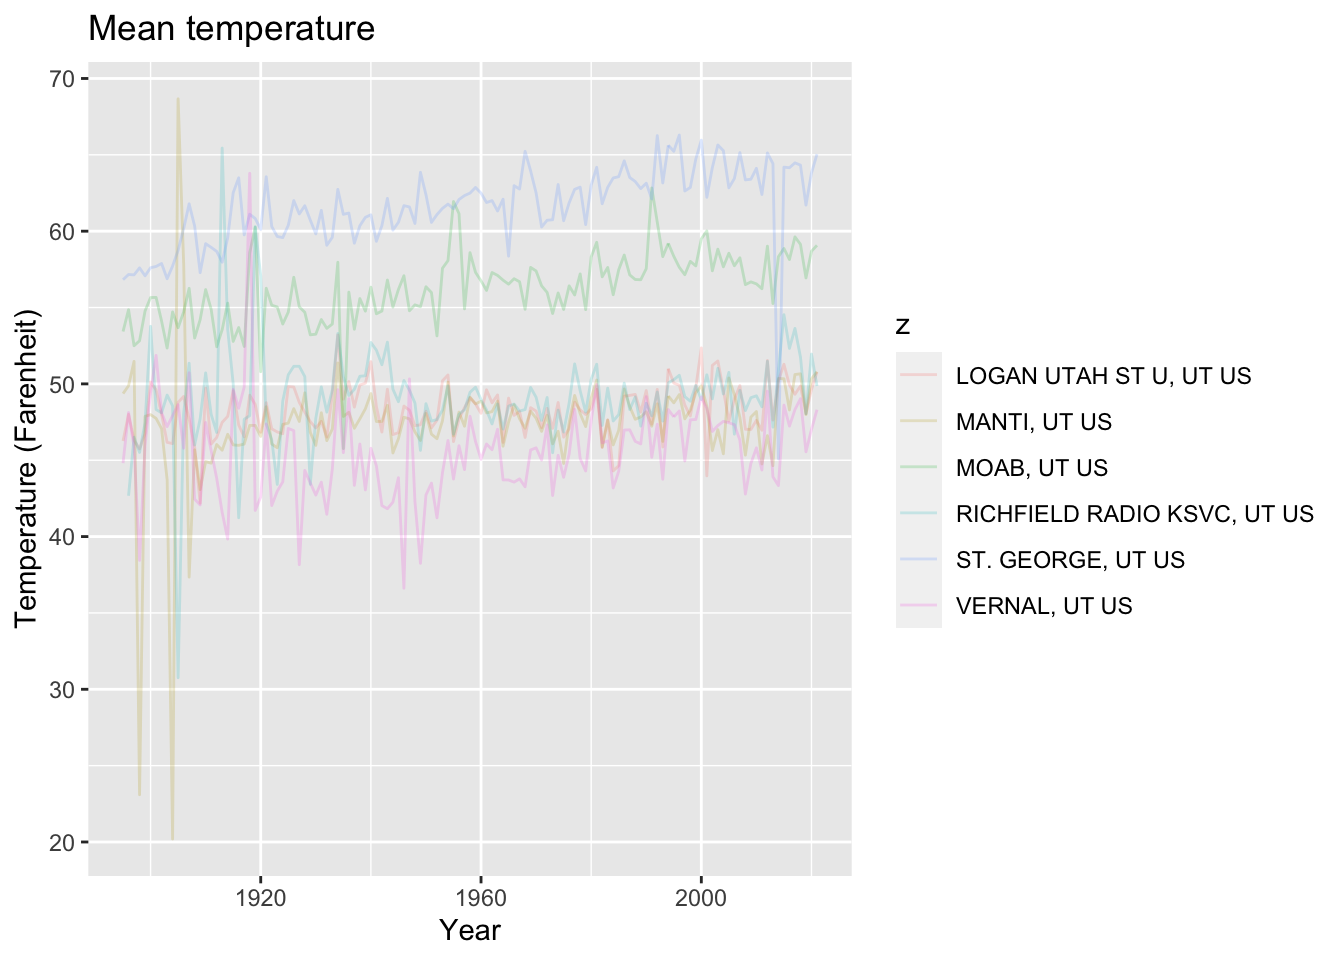
\includegraphics{Assignment3_files/figure-latex/unnamed-chunk-1-1.pdf}
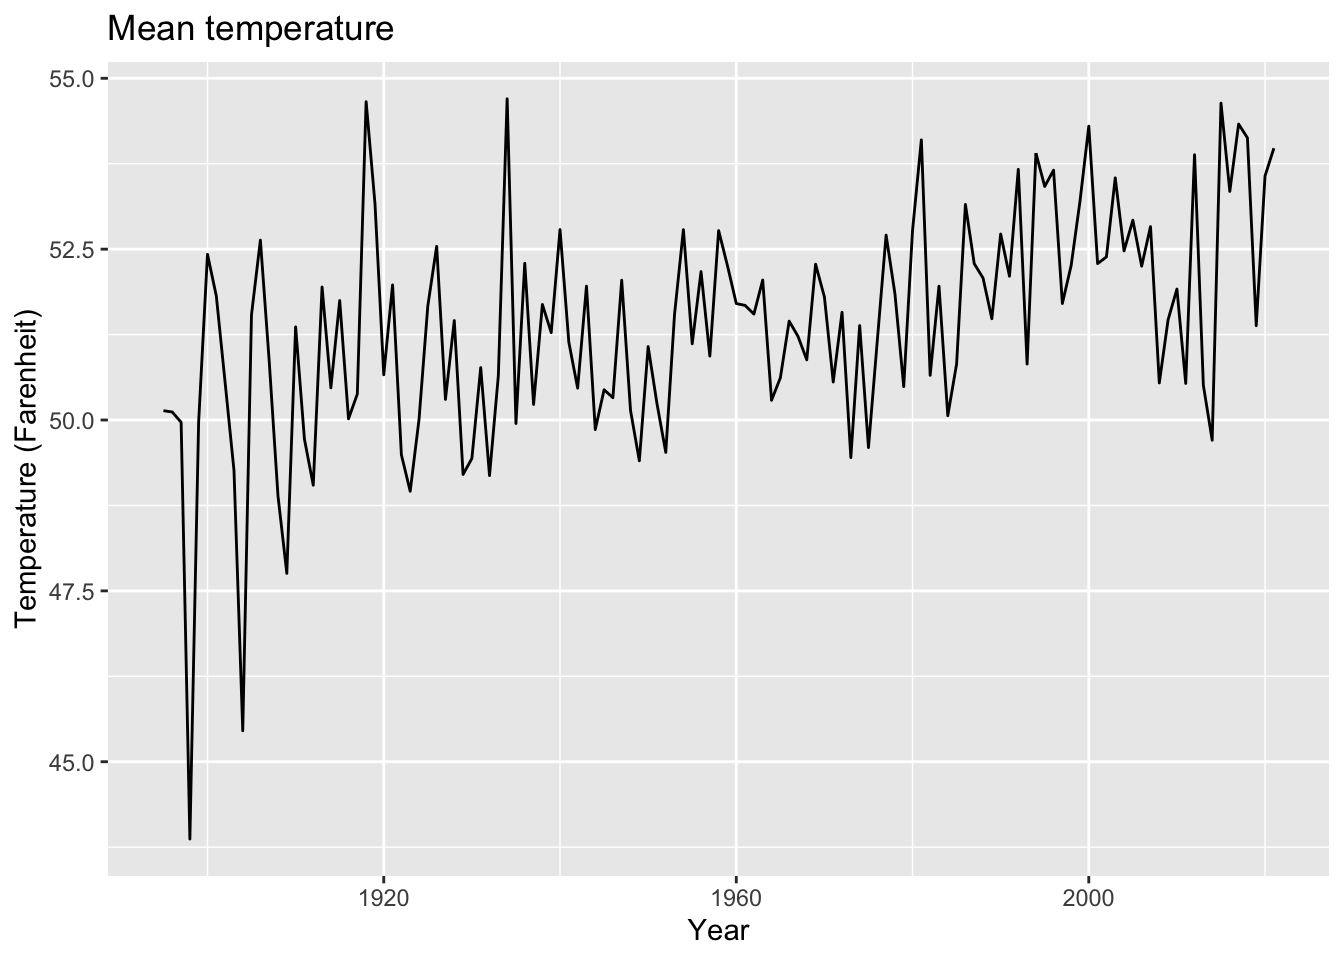
\includegraphics{Assignment3_files/figure-latex/unnamed-chunk-1-2.pdf}

We can immediately spot some serious outliers. Unfortunately, even the
highest coverage data still has some years where it has large gaps in
coverage (the gaps in coverage tend to be connected periods, not
isolated days -- possibly due to station issues). This leads to years
where the entire winter or summer is missing, which obviously largely
skews the data. Accounting for the missing data is challenging. Removing
any given station for a particular is out of the question -- some
stations (like St.~George) are much hotter, so removing them would skew
the years average colder. Replacing the stations data with it's
\emph{all-time} mean is better, but may still skew the data (if we only
have data from a very cold summer, doesn't that still mean the year
wasn't likely mean temperatures?). Extrapolating a mean temperature for
the year by comparing the data we do have to the same time period for
other years may be a good solution, but is beyond the capability of this
study. As such, we will simply replace missing days with the mean
temperature of \emph{that day} from all other years at that station.

Doing this substitution gives us the following:

\includegraphics{Assignment3_files/figure-latex/unnamed-chunk-2-1.pdf}
\includegraphics{Assignment3_files/figure-latex/unnamed-chunk-2-2.pdf}

We can see the effect that replacing missing data with the all-time mean
for that day has -- some high / low outlier years are moderate now.
There still appears to be some abnormal years -- Manti seems especially
cold in 1898, and Richfield seems especially hot in 1916. However,
seeing as these weren't caused by missing data, we're going to have to
assume our weather station data is correct.

Finally, we come to the conclusion that the \emph{coldest year on record
in Utah is 1898}, and the \emph{hottest year on record in Utah is 1934}.

\hypertarget{question-3-is-utah-drier-than-it-was-80-years-ago}{%
\subsection{Question 3: Is Utah drier than it was 80 years
ago?}\label{question-3-is-utah-drier-than-it-was-80-years-ago}}

We will use the same weather stations as in Question 1 and 2. They
provide a good sample, and will allow us to remain consistent. Weather
stations collect two notable statistics to compute dryness:
precipitation and evaporation amounts. Unfortunately, evaporation data
was not very consistently collected over the last 80 years. As such, we
will define how ``dry'' a given day is just by total precipitation
amount. We will define how dry a given year is by the mean of its days.
Similar to the methodology in Question 1 and 2, we will replace missing
days with the mean of \emph{that day} from all other years at that
station.

\includegraphics{Assignment3_files/figure-latex/unnamed-chunk-3-1.pdf}
\includegraphics{Assignment3_files/figure-latex/unnamed-chunk-3-2.pdf}

The precipitation graphs don't immediately reveal an obvious trend. We
can see, however, that precipitation varies a lot from year to year. We
can't just compare 1942 and 2021 to see if Utah is drier than it was 80
years ago. Instead, we will consider the data in the periods from
1942-1957 and 2006-2021. In order to compare the samples, we ran a Welch
Two Sample T-test with a 95\% confidence interval. Unfortunately, NOAA's
data is not a simple random sample. This will unquantifiably affect the
test. However, it should still be a good estimate since the weather
patterns is mostly independent and the data is likely fairly
representative. The test shows that we can be 95\% confident that the
difference in average precipitation between 1942-1957 and 2006-2021 is
{[}-0.006663485, 0.001145355{]}. This means that we can't be 95\%
confident that the Utah is wetter or drier than 80 years ago. As such,
we will conclude that \emph{there is not sufficient evidence to suggest
that Utah is drier today than 80 years ago}.

\hypertarget{question-4-what-is-the-average-low-temperature-in-salt-lake-city-in-january}{%
\subsection{Question 4: What is the average low temperature in Salt Lake
City in
January?}\label{question-4-what-is-the-average-low-temperature-in-salt-lake-city-in-january}}

This question is somewhat ambiguous. We will interpret it as asking for
the mean low temperature in Salt Lake of days in January in recent
history. For our purposes, we will define recent history as the last 10
years. We also have to consider what counts Salt Lake City. We will use
the NOAA defined region. This region has a wide variety of elevations,
which will dramatically affect temperature. As such, we will select
stations that we believe represents a good variety. However, there is no
guarantee this is really representative. T

Since we only want Salt Lake City, our old pool of stations is no longer
adequate. Instead, we will use the following stations:

\begin{itemize}
\tightlist
\item
  SNOWBIRD, UT US
\item
  BOUNTIFUL BENCH, UT US
\item
  HARDSCRABBLE, UT US
\item
  LOUIS MEADOW, UT US
\item
  PARLEY S SUMMIT, UT US
\end{itemize}

Since we only needed to cover the last 10 years, we were able to choose
all stations with 100\% coverage. This avoids having to account for the
missing data problem.

\includegraphics{Assignment3_files/figure-latex/unnamed-chunk-5-1.pdf}
\includegraphics{Assignment3_files/figure-latex/unnamed-chunk-5-2.pdf}

The mean temperature for Salt Lake in January is 20.87704 degrees
Fahrenheit. We computed a 95\% confidence interval for the data as
18.987 -- 22.767. This means that, assuming our data is representative
of Salt Lake, we can be 95\% sure that the mean temperature is between
\textasciitilde19 and \textasciitilde23 degrees.

\hypertarget{conclusions}{%
\subsection{Conclusions}\label{conclusions}}

From out study, we have decided:

\begin{enumerate}
\def\labelenumi{\arabic{enumi}.}
\tightlist
\item
  The coldest year on record in Utah is 1898
\item
  The hottest year on record in Utah is 1934
\item
  We saw insufficient evidence to conclude Utah is either wetter or
  drier than 80 years ago
\item
  The mean low temperature in Salt Lake is 20.87704, with a 95\%
  confidence interval between 18.987 -- 22.767.
\end{enumerate}

Hopefully this data can help inform the Federation of Utah Outdoor
Recreation and Utah residents in general.

\end{document}
